\documentclass[a4paper]{article}

\newcommand{\uuid}[1]{}%{{\texttt[#1]}}

\def\nr{4}
\def\nr_b{3}

\newcommand{\NR}{5}
%\newcommand{\NR_B}{6}

\usepackage{amsthm,amsmath}

\usepackage{graphicx}

\newcounter{myCount}

\newtheorem{Theorem}%
[myCount]{Teorema}

\newtheorem*{Cor}%comment
{Corollary}

\newtheorem{Lem}%comment [myCount]
{Lemma}

\newcommand\prerequisites[1]{{[Pre:#1]}}
\begin{document}
\section{test input}
%
Hello\input{latex_test3},\input{latex_test4}are you?

Double input my \input{latex_test3}!

\section{first}%comment
the number \nr_b

\begin{Theorem}[A  Theorem for {$I=]0,1[$}]\label{CT}
  The formula
\[ \int_I {\sin(c)} \hbox{is an \textbf{integral}}\]
\end{Theorem}

\begin{Cor}[A Corollary]\label{CC}
  The other formula
  \begin{equation}%
    \label{eq:CC}
    \int_{\cos(c)}
  \end{equation}
\end{Cor}
\begin{Lem}\label{lem:2}
  \prerequisites {\emph{that chap}}
  Then a Lemma citing the equation \ref{eq:CC} of the un-numbered Corollary \ref{CC}
\end{Lem}

\begin{Theorem}[Another Theorem]
  The formula
  \[ \int_I{e^{f^{g(x)}}} \ \textbf{d}x \]
  and a citation to the first Theorem \ref{CT}
\end{Theorem}

\section*{second $\int$}

\begin{center}
  include with extension PDF
  \\
  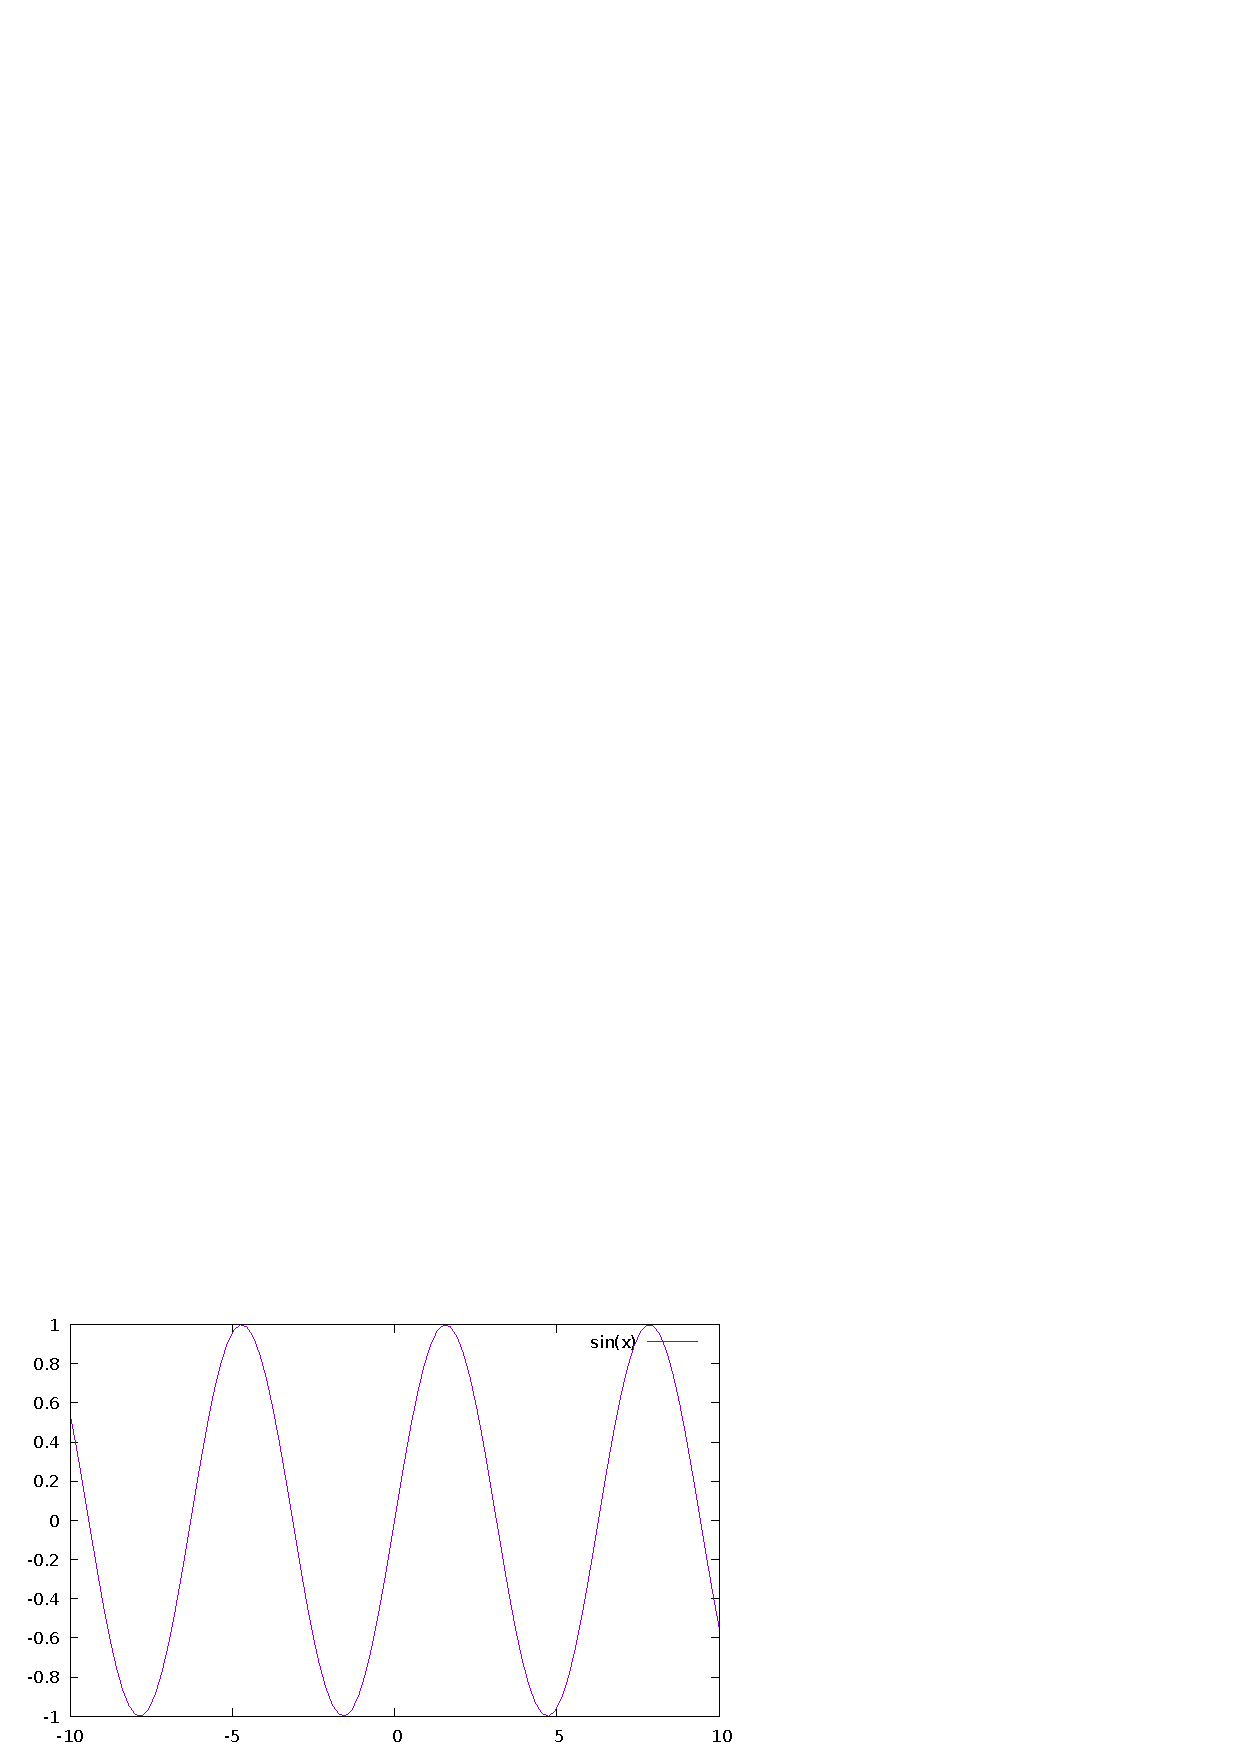
\includegraphics[width=0.5\textwidth]{F/sin.pdf}
  \\
  include with extension PNG
  \\
  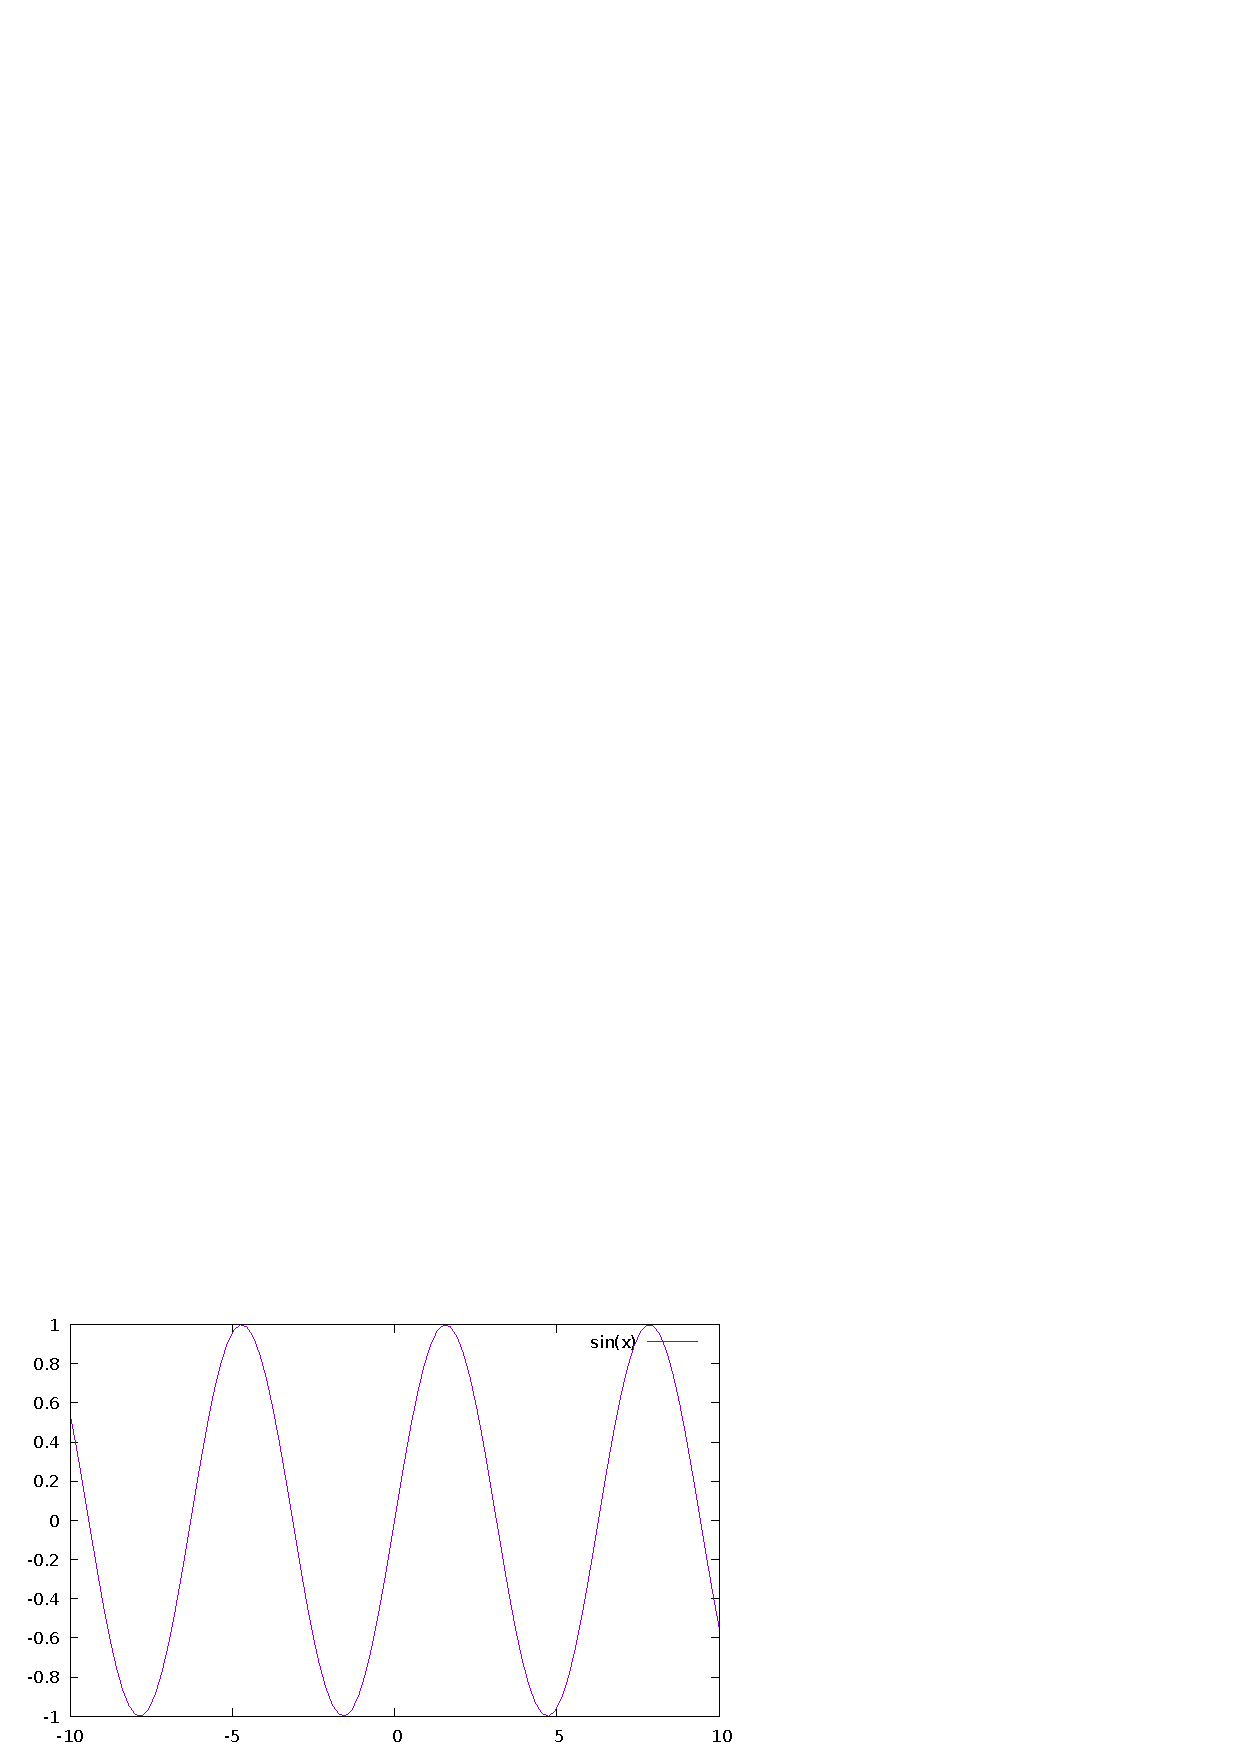
\includegraphics[width=0.5\textwidth]{F/sin.png}
  \\
  include smaller
  \\
  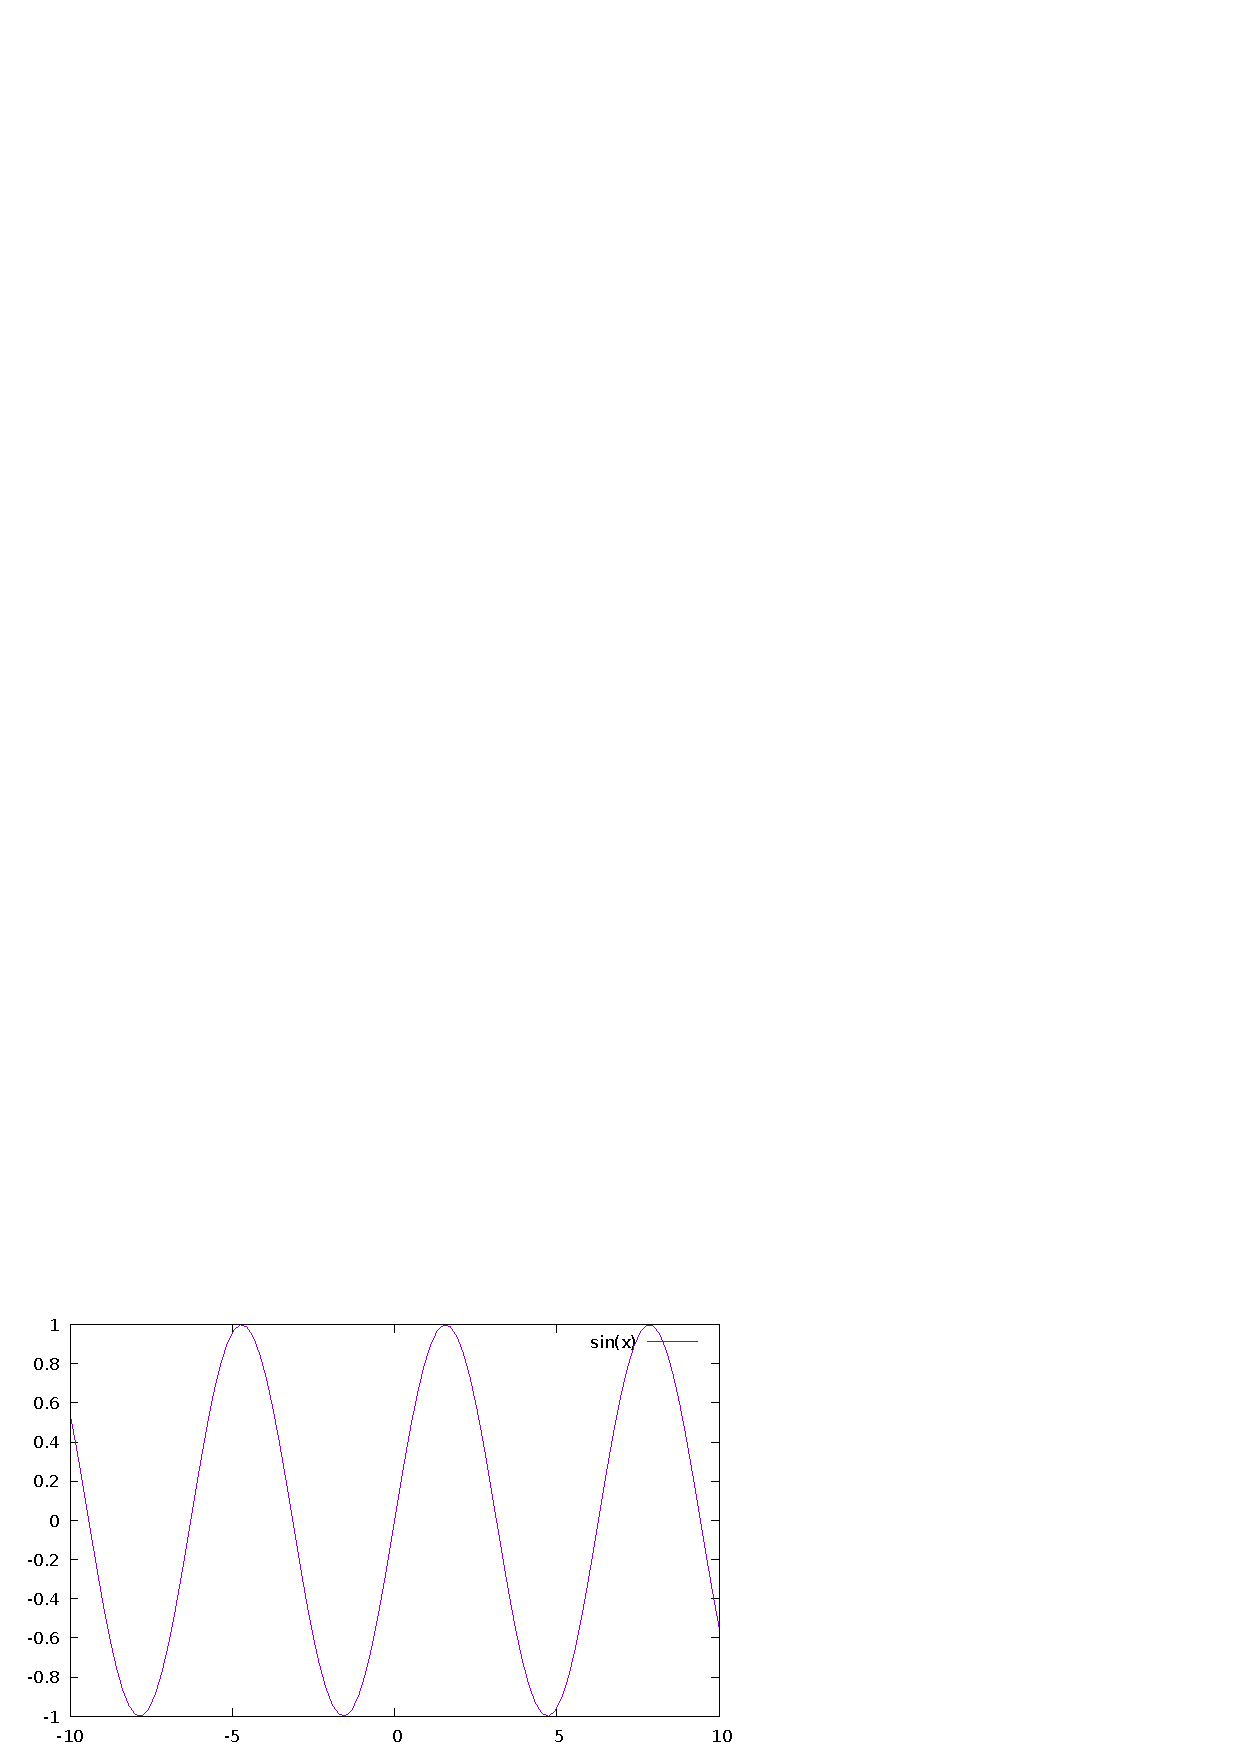
\includegraphics[width=0.2\textwidth]{F/sin.png}
  \\
  include without extension
  \\
  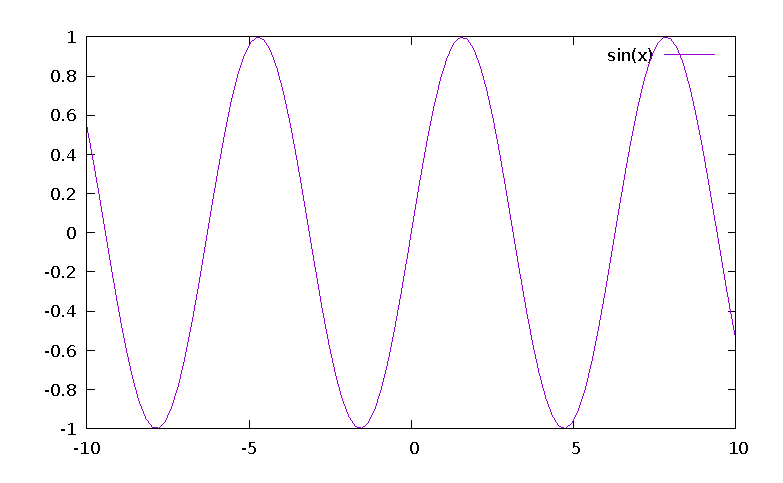
\includegraphics[width=0.5\textwidth]{F/sin}
\end{center}


a complex command
\emph{ital\`ic\textsl{~\~slanted\_\texttt{writer\_%
      \_macro}}}
\textbf{only boldface}

\begin{itemize}%comment

%comment

\item one
\item two
\end{itemize}


\begin{verbatim}
a verbatim
 \int_\label{343}
 \begin{Theorem}
\section*{A list inside an equation}%comment
yes you can
\begin{equation}
 \int \sin \quad \text{\fbox{\parbox{0.4\textwidth}{ is a simple integral that computes to   }}} =\cos
\end{equation}


%% TODO: neither `blob_inator` nor `plastex` currently support those weird latex constructs

%\begin{equation}
% \int \sin \quad \text{\fbox{\parbox{0.4\textwidth}{        \begin{itemize}
%       \item is a simple integral
%       \item it can be shown to be equal to
%       \end{itemize}
%  }}} =\cos
%\end{equation}

%\begin{equation}
% \int \sin \quad \text{ \input{textinequation} } =\cos
%\end{equation}



%%% Local Variables:
%%% mode: latex
%%% TeX-master: "latex_test1"
%%% End:

\input{UUID/pippo/pollo}
\end{verbatim}

\verb=a verbatim $\int$ and \input{UUID/nonexistent} =

%
\section*{A list inside an equation}%comment
yes you can
\begin{equation}
 \int \sin \quad \text{\fbox{\parbox{0.4\textwidth}{ is a simple integral that computes to   }}} =\cos
\end{equation}


%% TODO: neither `blob_inator` nor `plastex` currently support those weird latex constructs

%\begin{equation}
% \int \sin \quad \text{\fbox{\parbox{0.4\textwidth}{        \begin{itemize}
%       \item is a simple integral
%       \item it can be shown to be equal to
%       \end{itemize}
%  }}} =\cos
%\end{equation}

%\begin{equation}
% \int \sin \quad \text{ \input{textinequation} } =\cos
%\end{equation}



%%% Local Variables:
%%% mode: latex
%%% TeX-master: "latex_test1"
%%% End:

%

\section*{TOC}

\tableofcontents

\end{document}
